\newpage
\subsection{Motivación}

Los elementos de motivación se utilizan para modelar las motivaciones, o razones, que guían el diseño o el cambio de una Arquitectura Empresarial. Es esencial entender los factores, a menudo denominados impulsores, que influyen en otros elementos de motivación.  Pueden originarse tanto dentro como fuera de la empresa.  Los impulsores internos, también llamados preocupaciones, están asociados con las partes interesadas, que pueden ser algún ser humano individual o algún grupo de seres humanos, como un equipo de proyecto, una empresa o la sociedad. Ejemplos de esos impulsores internos son la satisfacción del cliente, el cumplimiento de la legislación o la rentabilidad. Es común que las empresas realicen una evaluación de esos factores impulsores; por ejemplo, utilizando un análisis FODA, a fin de responder de la mejor manera posible.

\begin{center}
	\begin{tabular}{ | m{6em} | m{4cm}| m{2cm} | } 
		\hline
		Motivación& Un elemento que proporciona el contexto o la razón detrás de la arquitectura de una empresa & 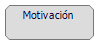
\includegraphics[width=0.8\linewidth, height=0.05\textheight]{imgs/Elementos/Motivacion.PNG}
		\\ 
		\hline
	\end{tabular}
\end{center}

\newpage
\subsubsection{Elementos de la Estructura}
\begin{table}[h!]
	\begin{center}
		\begin{tabular}{| m{6em} | m{7cm}| m{3cm} |}
			\hline
			Concepto & Descripción & Representación \\ 
			\hline
			
			Implicado 
			& 
			El papel de un individuo, equipo u organización (o clases de los mismos) que representa sus intereses en el resultado de la arquitectura 
			& 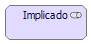
\includegraphics[width=0.8\linewidth, height=0.05\textheight]{imgs/Elementos/Implicado.PNG}
			\\
			\hline
			Manejador 
			& 
			Una condición externa o interna que motiva a una organización para definir sus galones e implementar los cambios necesarios para lograrlos. 
			& 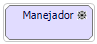
\includegraphics[width=0.8\linewidth, height=0.05\textheight]{imgs/Elementos/Manejador.PNG}
			\\
			\hline
			Valoración 
			& 
			El resultado de un análisis de la situación de la empresa con respecto a algún conductor. 
			& 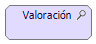
\includegraphics[width=0.8\linewidth, height=0.05\textheight]{imgs/Elementos/Valoracion.PNG}
			\\
			\hline
			Objetivo 
			& 
			Una declaración de intención, dirección o estado final deseado de alto nivel para una organización y sus partes interesadas. 
			& 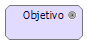
\includegraphics[width=0.8\linewidth, height=0.05\textheight]{imgs/Elementos/Objetivo.PNG}
			\\
			\hline
			Resultado 
			& 
			Un resultado final que se ha logrado
			& 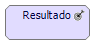
\includegraphics[width=0.8\linewidth, height=0.05\textheight]{imgs/Elementos/Resultado.PNG}
			\\
			\hline
			Principio 
			& 
			Una declaración cualitativa de intenciones que debe ser satisfecha por la arquitectura
			& 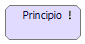
\includegraphics[width=0.8\linewidth, height=0.05\textheight]{imgs/Elementos/Principio.PNG}
			\\
			\hline
			Requerimiento 
			& 
			Una declaración de necesidad que debe ser satisfecha por la arquitectura
			& 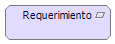
\includegraphics[width=0.8\linewidth, height=0.05\textheight]{imgs/Elementos/Requerimiento.PNG}
			\\
			\hline
			Restricción 
			& 
			Un factor que previene oUn factor que previene u obstruye laUn factor que previene u obstruye la realizaciónUn factor que previene u obstruye la realización de metas
			& 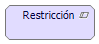
\includegraphics[width=0.8\linewidth, height=0.05\textheight]{imgs/Elementos/Restriccion.PNG}
			\\
			\hline
			Significado 
			& 
			Los conocimientos o la experiencia presentes en, o la interpretación dada a, un elemento
			& 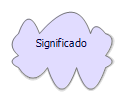
\includegraphics[width=0.8\linewidth, height=0.05\textheight]{imgs/Elementos/Significado.PNG}
			\\
			\hline
			Valor 
			& 
			El valor relativo, la utilidad o la importancia de un elemento básico o un resultado
			& 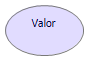
\includegraphics[width=0.8\linewidth, height=0.05\textheight]{imgs/Elementos/Valor.PNG}
			\\
			
			\hline
		\end{tabular}
		\caption{Conceptos Capa Motivacional}
		\label{tab:concepts}
	\end{center}
\end{table}